\documentclass[10pt,a4paper]{article}
\usepackage[latin1]{inputenc}
\usepackage{amsmath}
\usepackage{microtype}
\usepackage[none]{hyphenat}
\usepackage{verbatim}
\usepackage{amsfonts}
\usepackage{amssymb}
\usepackage{enumitem}
\renewcommand{\familydefault}{\sfdefault}
\usepackage{mathpazo}
\renewcommand{\rmdefault}{put}
\usepackage{enumitem}
\usepackage[dvipsnames,svgnames]{xcolor}
\usepackage{tkz-euclide}
\usetkzobj{all}
\usepackage{graphicx}
\usepackage{fancyhdr}
\usepackage{tikz} 	
\usepackage{adjustbox}
\usepackage{pgfplots}
\usepackage{multicol}
\usepackage{lipsum}
\usepackage[left=0.7cm,right=1cm,top=1cm,bottom=1.5cm]{geometry}
\usepackage{cancel} \usepackage{xcolor}
\usepackage{tcolorbox}
\usetikzlibrary{decorations.pathmorphing,patterns}
\usetikzlibrary{decorations.pathreplacing,calc}
 \newcommand\coret[2][red]{\renewcommand\CancelColor{\color{#1}}\cancel{#2}}
\SetLabelAlign{Center}{\hfil\makebox[1.0em]{#1}\hfil}

%%_------= solusi


% Set this =0 to hide, =1 to show

% Set this =0 to hide, =1 to show
\newtcolorbox{mybox}[1][] { colframe = blue!10, colback = blue!3,boxsep=0pt,left=0.2em, coltitle = blue!20!black, title = \textbf{jawab}, #1, } 

%---------- kunci (jika 1 ) muncul
\def\tampilkunci{0}
\newcommand{\hide}[1]{\ifnum\tampilkunci=1
%
\begin{mybox}
 #1
\end{mybox}
%
\vspace{\baselineskip}\fi\ifnum\tampilkunci=0
%
%\vspace{2cm}
%
\fi}



\newcommand*\cicled[1]{\tikz[baseline=(char.base)]{\node[white, shape=circle, fill=red!80,draw,inner sep=0.5pt](char){#1};}}

\newcommand*\kunci[1]{\ifnum\tampilkunci=1
%
\tikz[baseline=(char.base)]{\node[red, shape=circle,draw,inner sep=0.5pt,xshift=2pt](char){#1};}\stepcounter{enumii}
\fi\ifnum\tampilkunci=0
%
\hspace{3pt}#1\stepcounter{enumii}
%
\fi}

\newcommand*\silang[1]{\tikz[baseline=(char.base)]{
\draw[red,thick](-0.2,-0.20)--(0.2,0.2);
\draw[red,thick](-0.2,0.20)--(0.2,-0.2);
\node[black](char){#1};
}}

\newcommand*\centang[1]{\tikz[baseline=(char.base)]{
\draw[red, very thick](-0.2,0.1)--(-0.1,0)--(0.2,0.3);
\node(char){#1};
}}

\newcommand*\merah[1]{
\textcolor{red}{#1}}
\newcommand*\pilgan[1]{
\begin{enumerate}[label=\Alph*., itemsep=0pt,topsep=0pt,leftmargin=*,align=Center] #1 
\end{enumerate}}
\newcommand*\pernyataan[1]{
\begin{enumerate}[label=(\arabic*), itemsep=0pt,topsep=0pt,leftmargin=*] #1 
\end{enumerate}}
\pagestyle{fancy}
\renewcommand{\headrulewidth}{0pt}
\rfoot{\tiny{arifstwan}}
\newcommand{\pilgani}[1]{                            \vspace{-0.3cm}\begin{multicols}{2}
 \begin{enumerate}[label=\Alph*., itemsep=0pt,topsep=0pt,leftmargin=*,align=Center]#1                     \end{enumerate}
 \phantom{ini cuma sapi, wedus, dan ayam}
 \end{multicols}}


\begin{document}


 \textbf{Soal Gelombang Mekanik, berjalan} \phantom{ini nama siswa yang aaamengerjakan soal kuis ini }  

No callculator allowed !  
\begin{multicols*}{2}
\begin{enumerate}
% no1 ---------------------------------------------------------
\item Suatu gelombang memiliki persamaan $y = 3 \sin (8\pi t - 0,5\pi x)$, dengan satuan sekon dan meter. Maka panjang gelombang kecepatan rambat gelombang adalah . . . .
\pilgani{
    \item 2 m dan 2 m/s
    \item 4 m dan 3 m/s
    \item 2 m dan 3,5 m/s
    \item [\kunci{D.}] 4 m dan  16 m/s
    \item 4 m dan 12 m/s}
\hide{
    \begin{align*}
    v &=\frac{\omega}{k}\\
    v &=\frac{4\pi}{0,5\pi} = 8\text{ m/s}\\
    \phantom{a}
    \frac{2\pi}{\lambda}&= k\\
    \frac{2\pi}{\lambda} &=0.5\pi\\
    \lambda &= 4 \text{ m}
    \end{align*}
}
% no19  ---------------------------------------------------------
\item Perhatikan gambar gelombang berikut!

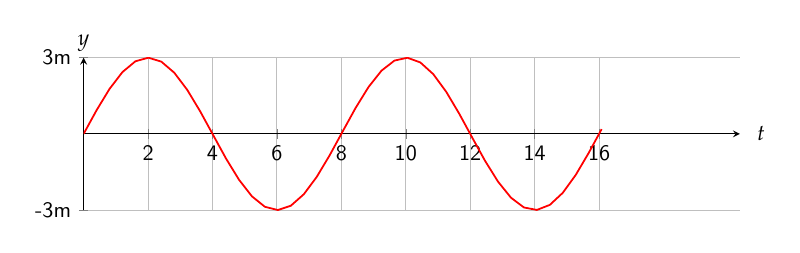
\begin{tikzpicture}[scale=0.8]
\begin{axis}[
   axis x line=center,
   ylabel={$y$},
   xlabel={$t$}, 
   axis y line=middle,
  every axis y label/.style={
          at={(ticklabel* cs:1.2)},
          anchor=north,},
   every axis x label/.style={
          at={(ticklabel* cs:1.05)},
          anchor=east,},
   xtick={0,1.5708,3.14159,...,14},
   xticklabels={0,2,...,16},
   ytick={-1,0,1},
   yticklabels={-3m, 0, 3m},
   xmin=.0, xmax=16,
   domain=0:4.02*pi, width=12cm,height=4cm,
   samples=41,grid]
  \addplot[thick, red, no marks] {sin(deg(x))};
  \end{axis}
  \end{tikzpicture}
  
  Jika panjang tali di atas adalah 8 m, maka persamaan gelombang yang tepat adalah . . .
   \pilgan{
     \item[\kunci{A.}] $y=3 \sin(0,25\pi t -0,5\pi x)$
     \item $y=6 \sin(0,25\pi t -0,5\pi x)$ 
     \item $y=3 \sin(0,5\pi t -0,5\pi x)$
     \item $y=6 \sin(0,5\pi t -0,25\pi x)$
     \item $y=3 \sin(0,25\pi t -0,25\pi x)$
}
\hide{
    Pesamaan gelombang $y=A sin (\omega t - kx)$ maka 
    \begin{align*}
    f &= \frac{n}{t} =\frac{2}{16}=\frac{1}{8}\\
    2\lambda &= 8 m\\
    \lambda &= 4 m\\
    \phantom{a}\\
    y  &= 3 \sin(2\pi\frac{1}{8} t - \frac{2\pi}{4}x)\\
    y &= 3 \sin(0,25\pi t - 0,5 \pi x)
    \end{align*}
}




% no20  ---------------------------------------------------------
\item Perhatikan gambar gelombang berikut!

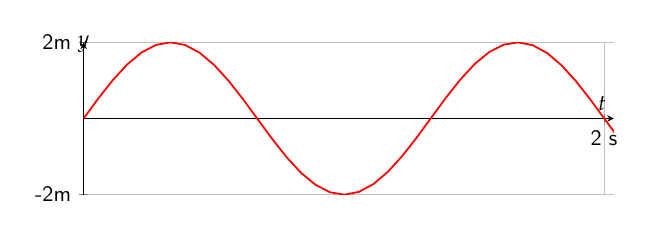
\begin{tikzpicture}[scale=0.8]
\begin{axis}[
   axis x line=center,
   ylabel={$y$},
   xlabel={$t$}, 
   axis y line=middle,
   every axis y label/.style={at={(current axis.north west)},above=2mm}, 
   xtick={0,9.42 },
   xticklabels={0,{2 s}},
   ytick={-1,0,1},
   yticklabels={-2m, 0,2m},
   xmin=.0, xmax=9.6,
   domain=0:3.34*pi, width=10cm,height=4cm,
   samples=41,grid]
  \addplot[thick, red, no marks] {sin(deg(x))};
  \end{axis}
  \end{tikzpicture}
  
  Jika panjang tali di atas adalah 12 m, maka persamaan gelombang yang tepat adalah . . .
   \pilgan{
         \item $y=4 \sin(0,25\pi t -0,5\pi x)$ 
      \item[\kunci{B.}] $y=2 \sin(1,5\pi t -0,25\pi x)$
     \item $y=4 \sin(0,5\pi t -0,5\pi x)$
     \item $y=2 \sin(0,5\pi t -0,25\pi x)$
     \item $y=2 \sin(0,25\pi t -0,25\pi x)$
}
\hide{
Gunakan cara seperti gambar sebelumnya  
}




% no21  ---------------------------------------------------------
\item Suatu gelombang memiliki persamaan $y=4 \sin(0,2\pi x) \cos (3\pi t)$, panjang gelombang dan jenis gelombangnya adalah . . .
\pilgan{
	\item 4 m dan stasioner ujung bebas
	\item[\kunci{B.}] 10 m dan stasioner ujung terikat
	\item 10m dan stasioner ujung bebas
	\item 4 m dan stasioner ujung terikat
	\item 4 m dan berjalan }
\hide{
Aturan sederhana

jika $x$ dalam aturan sinus maka ujung terikat 

jika $x$ dalam aturan cos maka ujung bebas

Pada soal $\sin(0,2\pi x)$, maka ujung terikat. Mencari panjang gelombang dengan
\begin{align*}
k&= \frac{2 \pi}{\lambda}\\
0,2 \pi &= \frac{2\pi}{\lambda}\\
\lambda &= 10 \text { m}
\end{align*}

}





% no22  ---------------------------------------------------------
\item Suatu gelombang memiliki persamaan $y=4 \sin(0,2\pi x) \cos (4\pi t)$, kecepatan rambat gelombang adalah . . . 
\pilgani{
	\item 2 m/s
	\item 0,5 m/s
	\item 0,4 m/s
	\item [\kunci{D.}] 20 m/s
	\item 10 m/s
	}
\hide{kecepatan pada persamaan gelombang bisa dikerjakan dengan menggunakan $\omega$ dan $k$ secara langsung
\begin{align*}
v&=\frac{\omega}{k}\\
v &= \frac{4\coret{\pi}}{0,2\coret{\pi}}\
v & = 20 \text{ m/s}
\end{align*}

}





% no23  ---------------------------------------------------------
\item  Persamaan gelombang adalah $y=4 \cos (2\pi t) \sin( 0,1 \pi x)$. Jarak simpul ke-3 dari ujung getar adalah . . .
\pilgani{
        \item 4 m
        \item 0,1 m
        \item 0,5 m
        \item 10 m
        \item 20 m }
\hide{ Berdasarkan aturan sebelumnya, ini adalah gelombang ujung terikat. tentukan $\lambda$
\begin{align*}
k &=\frac{2\pi}{\lambda}\\
0,1\pi & = \frac{2\pi}{\lambda}\\
\lambda &= 20 \text{ m}
\end{align*}

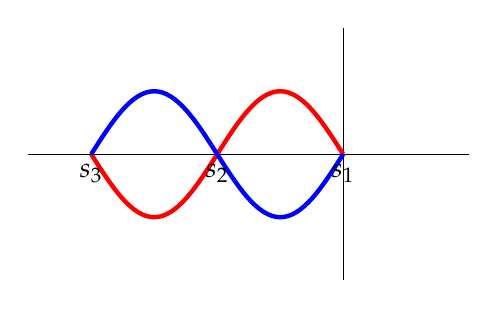
\begin{tikzpicture}[scale=0.8]
\draw(-5,0) -- (2,0) ;
\draw(0,-2)--(0,2);
\draw[ultra thick, red] (0,0) sin (-1,1) cos (-2,0) sin (-3,-1) cos (-4,0);
\draw[ultra thick, blue] (0,0) sin (-1,-1) cos (-2,0) sin (-3,1) cos (-4,0);
\foreach \x/\y in {0/{$s_1$},-2/{$s_2$},-4/{$s_3$}}{
\node at (\x,-0.3cm){\y};}
\end{tikzpicture}

Karena $s_3$ jaraknya adalah 1 gelombang, maka $s_3$= 20 m}

% no24  ---------------------------------------------------------
\item Persamaan getar suatu gelombang adalah $y=8\sin(8\pi t) \cos (0,4 \pi x ) $. Jarak simpul pertama dan perut ketiga adalah . . .
\pilgani{
        \item [\kunci{A.}]$\frac{15}{4}$ m 
        \item 2 m
        \item 5 m 
        \item 8 m 
        \item 10 m 
        }
\hide { Gambar dulu seperti gambar di atas. Karena $\cos(kx)$ maka ujung bebas

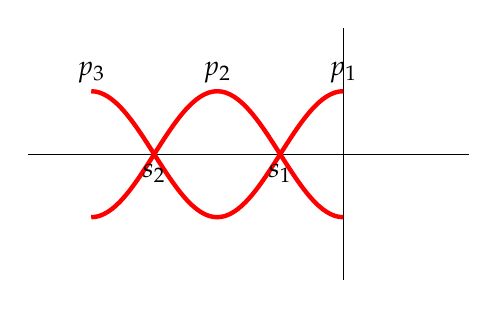
\begin{tikzpicture}[scale=0.8]
\draw(-5,0) -- (2,0) ;
\draw(0,-2)--(0,2);
\draw[ultra thick, red] (0,1) cos (-1,0) sin (-2,-1) cos (-3,0) sin (-4,1);
\draw[ultra thick, red] (0,-1) cos (-1,0) sin (-2,1) cos (-3,0) sin (-4,-1);

\foreach \x/\y in {0/{$p_1$},-2/{$p_2$},-4/{$p_3$}}{
\node at (\x,1.3cm){\y};}

\foreach \x/\y in {-1/{$s_1$},-3/{$s_2$}}{
\node at (\x,-0.3cm){\y};}

\end{tikzpicture}

Jarak $s_1$ ke $p_3$ adalah $\frac{3}{4} \lambda$ maka $s=\frac{3}{4}\times 5=\frac{15}{4}$ m



}



% no25  ---------------------------------------------------------
\item Persamaan getar suatu gelombang adalah $y=8\sin(8\pi t) \cos (0,4 \pi x ) $. Periode gelombang tersebut adalah . . .
\pilgani{
        \item 4 s
        \item[\kunci{B.}] 0,25 s
        \item 0,5 s
        \item 1 s
        \item 2 s
        }
\hide { $\omega = 2\pi f$ maka frekuensi adalah 4 Hz. Sehingga periodenya 1/$f$ = 0,25 s }




% no26  ---------------------------------------------------------
\item Persamaan getar suatu gelombang adalah $y=8\sin(8\pi t) \cos (0,4 \pi x ) $. Kecepatan rambat gelombang tersebut adalah . . .
\pilgani{
        \item [\kunci{A.}] 20 m/s
        \item 40 m/s
        \item 50 m/s
        \item 80 m/s
        \item 10 m/s
        }
\hide{Kecepatan rambat 
\begin{align*}
v&=\frac{\omega}{k}\\
v&=\frac{8\pi}{0,4\pi}\\
v&=20 \text{ m/s}
\end{align*}}



% no27  ---------------------------------------------------------
\item Suatu gelombang dengan persamaan $y=4\sin(4\pi t) \cos (0,5\pi x)$. Jarak simpul ketiga dari titik pantul . . . .
\pilgani{
        \item 2 m
        \item 3 m
        \item 5/4 m
        \item 4 m
        \item [\kunci{E.}]5 m}

\hide{ silakan gambar seperti yang sebelumnya}


% no28  ---------------------------------------------------------
\item Suatu gelombang dengan persamaan $y=4\sin(4\pi t) \cos (0,5\pi x)$. Jarak perut ke 1 dari titik pantul adalah . . .
\pilgani{ 
        \item [\kunci{A.}] 0 m
        \item 5/4 m
        \item 4 m
        \item 5 m
        \item 3 m
        }
\hide{ silakan gambar seperti yang sebelumnya}






% no29  ---------------------------------------------------------
\item Suatu gelombang dengan persamaan $y=4\sin(4\pi t) \cos (0,5\pi x)$. Amplitudo sumber gelombang adalah . . . . 
\pilgani{
        \item 1 m
        \item[\kunci{B.}] 2 m
        \item 3 m
        \item 4 m
        \item tidak ada
        }
\hide{ silakan gambar seperti yang sebelumnya}






% no30  ---------------------------------------------------------
\item Suatu gelombang dengan persamaan $y=4\sin(4\pi t) \cos (0,5\pi x)$. Simpangan di titik dengan jarak 2/3 m pada saat $t=\frac{1}{12}$ s adalah . . .
\pilgani{
        \item[\kunci{A.}] $\sqrt{3}$
        \item 2 $\sqrt{3}$
        \item 2 
        \item 4
        \item 2 $\sqrt{2}$}

\hide{masukan nilai $t$ dan $x$ dalam persamaan, sehingga
\begin{align*}
y&=4\sin(4\pi t) \cos (0,5\pi x)\\
y&=4\sin(4\pi \frac{1}{12})\cos(0,5\pi \frac{2}{3})\\
y&= 4 \sin(\frac{\pi}{3})\cos(\frac{\pi}{3})\\
y&=4.\frac{1}{2}\sqrt{3}\frac{1}{2}\\
y&=\sqrt{3}
\end{align*}
}







% no31 ---------------------------------------------------------
\item Pengaruh memperbesar amplitudo terhadap bunyi adalah . . . 
\pilgani{
	\item [\kunci{A.}] Suara semakin keras (volume)
	\item Frekuensi makin tinggi
	\item frekuensi rendah
	\item taraf intensitas semakin rendah
	\item butuh energi lebih rendah}
\hide{ Amplitudo membutuhkan energi lebih tinggi, selain itu semakin besar amplitudo suara semakin keras (intensitas semakin tinggi) }

% no31.b ----------------------------------------------------------
\item[31.b] Pengaruh frekuensi bunyi yang semakin tinggi adalah . . . (hint: $v=\lambda . f$)
\pilgani{
	\item kecepatan semakin besar
	\item panjang gelombang makin besar
	\item[\kunci{C.}] panjang gelombang makin pendek
	\item suara makin kuat (keras) 
	\item taraf intensitas makin besar
}
\hide{Kecepatan bunyi pada suatu keadaan (misal di medium udara) akan tetap selama faktor2 tetap. Faktor tersebut misalnya (gaya pada tali, massa jenis tali, massa jenis medium, dsb). 

Jadi saat frekuensi naik panjang gelombangnya yang semaki kecil}

% no31.c ---------------------------------------------------------------------

% no32 ---------------------------------------------------------
\item Kuningan memiliki massa jennis 8400 kg/m$^3$. Pada suatu kabel dengan bahan kuningan dan memiliki modulus elastisitas sebesar 2,1 x  10$^9$ N/m$^2$, maka kecepatan suara pada kuningan tersebut adalah . .. 
\pilgani{
	\item 300 m/s
	\item 250 m/s
	\item[\kunci{C.}] 500 m/s
	\item 420 m/s
	\item 600 m/s }
\hide{ 
\begin{align*}
v&=\sqrt{\frac{E}{\rho}}\\
\phantom{a}\\
E&: \text{ Modulus elastisitas/young}\\
\rho &: \text{ Massa jenis zat}\\
\phantom{a}\\
v &= \sqrt{\frac{2,1\times 10^9}{8400}}\\
v& =\sqrt{250000}=500 \text{ m/s}
\end{align*} }


% no33 ---------------------------------------------------------
\item Perhatikan pernyataan berikut tentang pernyataan melde
\pernyataan{
	\item Memperpanjang tali
	\item mengubah tali dengan massa jenis lebih kecil
	\item mengubah beban dengan yang lebih besar
	\item memendekan talli
	}
Usaha yang dapat dilakukan untuk meningkatkan frekuensi adalah . . . ({ hint: frekuensi sebanding dengan kecepatan})
\pilgani{
	\item 1,3
	\item 1,2,3
	\item [\kunci{C.}]2,3,4
	\item 2,4
	\item 4 saja}
\hide{Lihat rumus pada soal no 34}


% no33.b -------------------------------------------------------
\item Cepat rambat gelombang pada tali dituliskan pada rumus
$$ v = \sqrt{\frac{F.l}{m}} =\sqrt{\frac{F}{\mu}} $$
Suatu tali dengan massa 10 gram dan panjang 2 m digantungi beban dengan massa 800 gram. Maka kecepatan getar pada tali tersebut adalah . . . 
\pilgani{
    \item 10 m/s
    \item 20 m/s
    \item [\kunci{C.}]40 m/s
    \item 50 m/s
    \item 100 m/s}
\hide{
    Pada soal tersebut sudah jelas bahwa kecepatan tinggal masukan pada persamaan, sehingga
    \begin{align*}
    v& =\sqrt{\frac{F.l}{m}}\\
    v&=\sqrt{\frac{8.2}{0,01}}=\sqrt{1600}=40\text{ m/s}
    \end{align*}
}

\end{enumerate}
\end{multicols*} \end{document} 

